% Options for packages loaded elsewhere
\PassOptionsToPackage{unicode}{hyperref}
\PassOptionsToPackage{hyphens}{url}
\PassOptionsToPackage{dvipsnames,svgnames,x11names}{xcolor}
%
\documentclass[
]{article}

\usepackage{amsmath,amssymb}
\usepackage{iftex}
\ifPDFTeX
  \usepackage[T1]{fontenc}
  \usepackage[utf8]{inputenc}
  \usepackage{textcomp} % provide euro and other symbols
\else % if luatex or xetex
  \usepackage{unicode-math}
  \defaultfontfeatures{Scale=MatchLowercase}
  \defaultfontfeatures[\rmfamily]{Ligatures=TeX,Scale=1}
\fi
\usepackage{lmodern}
\ifPDFTeX\else  
    % xetex/luatex font selection
\fi
% Use upquote if available, for straight quotes in verbatim environments
\IfFileExists{upquote.sty}{\usepackage{upquote}}{}
\IfFileExists{microtype.sty}{% use microtype if available
  \usepackage[]{microtype}
  \UseMicrotypeSet[protrusion]{basicmath} % disable protrusion for tt fonts
}{}
\makeatletter
\@ifundefined{KOMAClassName}{% if non-KOMA class
  \IfFileExists{parskip.sty}{%
    \usepackage{parskip}
  }{% else
    \setlength{\parindent}{0pt}
    \setlength{\parskip}{6pt plus 2pt minus 1pt}}
}{% if KOMA class
  \KOMAoptions{parskip=half}}
\makeatother
\usepackage{xcolor}
\setlength{\emergencystretch}{3em} % prevent overfull lines
\setcounter{secnumdepth}{5}
% Make \paragraph and \subparagraph free-standing
\makeatletter
\ifx\paragraph\undefined\else
  \let\oldparagraph\paragraph
  \renewcommand{\paragraph}{
    \@ifstar
      \xxxParagraphStar
      \xxxParagraphNoStar
  }
  \newcommand{\xxxParagraphStar}[1]{\oldparagraph*{#1}\mbox{}}
  \newcommand{\xxxParagraphNoStar}[1]{\oldparagraph{#1}\mbox{}}
\fi
\ifx\subparagraph\undefined\else
  \let\oldsubparagraph\subparagraph
  \renewcommand{\subparagraph}{
    \@ifstar
      \xxxSubParagraphStar
      \xxxSubParagraphNoStar
  }
  \newcommand{\xxxSubParagraphStar}[1]{\oldsubparagraph*{#1}\mbox{}}
  \newcommand{\xxxSubParagraphNoStar}[1]{\oldsubparagraph{#1}\mbox{}}
\fi
\makeatother

\usepackage{color}
\usepackage{fancyvrb}
\newcommand{\VerbBar}{|}
\newcommand{\VERB}{\Verb[commandchars=\\\{\}]}
\DefineVerbatimEnvironment{Highlighting}{Verbatim}{commandchars=\\\{\}}
% Add ',fontsize=\small' for more characters per line
\usepackage{framed}
\definecolor{shadecolor}{RGB}{241,243,245}
\newenvironment{Shaded}{\begin{snugshade}}{\end{snugshade}}
\newcommand{\AlertTok}[1]{\textcolor[rgb]{0.68,0.00,0.00}{#1}}
\newcommand{\AnnotationTok}[1]{\textcolor[rgb]{0.37,0.37,0.37}{#1}}
\newcommand{\AttributeTok}[1]{\textcolor[rgb]{0.40,0.45,0.13}{#1}}
\newcommand{\BaseNTok}[1]{\textcolor[rgb]{0.68,0.00,0.00}{#1}}
\newcommand{\BuiltInTok}[1]{\textcolor[rgb]{0.00,0.23,0.31}{#1}}
\newcommand{\CharTok}[1]{\textcolor[rgb]{0.13,0.47,0.30}{#1}}
\newcommand{\CommentTok}[1]{\textcolor[rgb]{0.37,0.37,0.37}{#1}}
\newcommand{\CommentVarTok}[1]{\textcolor[rgb]{0.37,0.37,0.37}{\textit{#1}}}
\newcommand{\ConstantTok}[1]{\textcolor[rgb]{0.56,0.35,0.01}{#1}}
\newcommand{\ControlFlowTok}[1]{\textcolor[rgb]{0.00,0.23,0.31}{\textbf{#1}}}
\newcommand{\DataTypeTok}[1]{\textcolor[rgb]{0.68,0.00,0.00}{#1}}
\newcommand{\DecValTok}[1]{\textcolor[rgb]{0.68,0.00,0.00}{#1}}
\newcommand{\DocumentationTok}[1]{\textcolor[rgb]{0.37,0.37,0.37}{\textit{#1}}}
\newcommand{\ErrorTok}[1]{\textcolor[rgb]{0.68,0.00,0.00}{#1}}
\newcommand{\ExtensionTok}[1]{\textcolor[rgb]{0.00,0.23,0.31}{#1}}
\newcommand{\FloatTok}[1]{\textcolor[rgb]{0.68,0.00,0.00}{#1}}
\newcommand{\FunctionTok}[1]{\textcolor[rgb]{0.28,0.35,0.67}{#1}}
\newcommand{\ImportTok}[1]{\textcolor[rgb]{0.00,0.46,0.62}{#1}}
\newcommand{\InformationTok}[1]{\textcolor[rgb]{0.37,0.37,0.37}{#1}}
\newcommand{\KeywordTok}[1]{\textcolor[rgb]{0.00,0.23,0.31}{\textbf{#1}}}
\newcommand{\NormalTok}[1]{\textcolor[rgb]{0.00,0.23,0.31}{#1}}
\newcommand{\OperatorTok}[1]{\textcolor[rgb]{0.37,0.37,0.37}{#1}}
\newcommand{\OtherTok}[1]{\textcolor[rgb]{0.00,0.23,0.31}{#1}}
\newcommand{\PreprocessorTok}[1]{\textcolor[rgb]{0.68,0.00,0.00}{#1}}
\newcommand{\RegionMarkerTok}[1]{\textcolor[rgb]{0.00,0.23,0.31}{#1}}
\newcommand{\SpecialCharTok}[1]{\textcolor[rgb]{0.37,0.37,0.37}{#1}}
\newcommand{\SpecialStringTok}[1]{\textcolor[rgb]{0.13,0.47,0.30}{#1}}
\newcommand{\StringTok}[1]{\textcolor[rgb]{0.13,0.47,0.30}{#1}}
\newcommand{\VariableTok}[1]{\textcolor[rgb]{0.07,0.07,0.07}{#1}}
\newcommand{\VerbatimStringTok}[1]{\textcolor[rgb]{0.13,0.47,0.30}{#1}}
\newcommand{\WarningTok}[1]{\textcolor[rgb]{0.37,0.37,0.37}{\textit{#1}}}

\providecommand{\tightlist}{%
  \setlength{\itemsep}{0pt}\setlength{\parskip}{0pt}}\usepackage{longtable,booktabs,array}
\usepackage{calc} % for calculating minipage widths
% Correct order of tables after \paragraph or \subparagraph
\usepackage{etoolbox}
\makeatletter
\patchcmd\longtable{\par}{\if@noskipsec\mbox{}\fi\par}{}{}
\makeatother
% Allow footnotes in longtable head/foot
\IfFileExists{footnotehyper.sty}{\usepackage{footnotehyper}}{\usepackage{footnote}}
\makesavenoteenv{longtable}
\usepackage{graphicx}
\makeatletter
\newsavebox\pandoc@box
\newcommand*\pandocbounded[1]{% scales image to fit in text height/width
  \sbox\pandoc@box{#1}%
  \Gscale@div\@tempa{\textheight}{\dimexpr\ht\pandoc@box+\dp\pandoc@box\relax}%
  \Gscale@div\@tempb{\linewidth}{\wd\pandoc@box}%
  \ifdim\@tempb\p@<\@tempa\p@\let\@tempa\@tempb\fi% select the smaller of both
  \ifdim\@tempa\p@<\p@\scalebox{\@tempa}{\usebox\pandoc@box}%
  \else\usebox{\pandoc@box}%
  \fi%
}
% Set default figure placement to htbp
\def\fps@figure{htbp}
\makeatother

\usepackage{booktabs}
\usepackage{caption}
\usepackage{longtable}
\usepackage{colortbl}
\usepackage{array}
\usepackage{anyfontsize}
\usepackage{multirow}
\makeatletter
\@ifpackageloaded{caption}{}{\usepackage{caption}}
\AtBeginDocument{%
\ifdefined\contentsname
  \renewcommand*\contentsname{Table of contents}
\else
  \newcommand\contentsname{Table of contents}
\fi
\ifdefined\listfigurename
  \renewcommand*\listfigurename{List of Figures}
\else
  \newcommand\listfigurename{List of Figures}
\fi
\ifdefined\listtablename
  \renewcommand*\listtablename{List of Tables}
\else
  \newcommand\listtablename{List of Tables}
\fi
\ifdefined\figurename
  \renewcommand*\figurename{Figure}
\else
  \newcommand\figurename{Figure}
\fi
\ifdefined\tablename
  \renewcommand*\tablename{Table}
\else
  \newcommand\tablename{Table}
\fi
}
\@ifpackageloaded{float}{}{\usepackage{float}}
\floatstyle{ruled}
\@ifundefined{c@chapter}{\newfloat{codelisting}{h}{lop}}{\newfloat{codelisting}{h}{lop}[chapter]}
\floatname{codelisting}{Listing}
\newcommand*\listoflistings{\listof{codelisting}{List of Listings}}
\makeatother
\makeatletter
\makeatother
\makeatletter
\@ifpackageloaded{caption}{}{\usepackage{caption}}
\@ifpackageloaded{subcaption}{}{\usepackage{subcaption}}
\makeatother

\usepackage{bookmark}

\IfFileExists{xurl.sty}{\usepackage{xurl}}{} % add URL line breaks if available
\urlstyle{same} % disable monospaced font for URLs
\hypersetup{
  pdftitle={Umbria},
  pdfauthor={Lorenzo Mattioli},
  colorlinks=true,
  linkcolor={blue},
  filecolor={Maroon},
  citecolor={Blue},
  urlcolor={Blue},
  pdfcreator={LaTeX via pandoc}}


\title{Umbria}
\author{Lorenzo Mattioli}
\date{}

\begin{document}
\maketitle

\renewcommand*\contentsname{Table of contents}
{
\hypersetup{linkcolor=}
\setcounter{tocdepth}{3}
\tableofcontents
}

\section{Introduzione}\label{introduzione}

Due parole sull'Umbria

\section{Analisi della struttura per
età}\label{analisi-della-struttura-per-etuxe0}

\subsection{Piramidi delle età}\label{piramidi-delle-etuxe0}

\begin{Shaded}
\begin{Highlighting}[]
\DocumentationTok{\#\# Italia {-}{-}{-}{-}}
\DocumentationTok{\#\#\# 2024}
\NormalTok{it24gg }\OtherTok{\textless{}{-}}\NormalTok{ it24 }\SpecialCharTok{|\textgreater{}} 
  \FunctionTok{filter}\NormalTok{(Sesso }\SpecialCharTok{!=} \StringTok{\textquotesingle{}Totale\textquotesingle{}}\NormalTok{) }\SpecialCharTok{|\textgreater{}}
  \FunctionTok{ggplot}\NormalTok{(}\FunctionTok{aes}\NormalTok{(}\AttributeTok{x =}\NormalTok{ Età,}
             \AttributeTok{y =} \FunctionTok{ifelse}\NormalTok{(Sesso }\SpecialCharTok{==} \StringTok{\textquotesingle{}M\textquotesingle{}}\NormalTok{,}
                        \SpecialCharTok{{-}}\StringTok{\textasciigrave{}}\AttributeTok{Tot per genere}\StringTok{\textasciigrave{}}\NormalTok{, }\StringTok{\textasciigrave{}}\AttributeTok{Tot per genere}\StringTok{\textasciigrave{}}\NormalTok{),}
             \AttributeTok{fill =}\NormalTok{ Sesso)) }\SpecialCharTok{+}
  \FunctionTok{geom\_bar}\NormalTok{(}\AttributeTok{stat =} \StringTok{\textquotesingle{}identity\textquotesingle{}}\NormalTok{, }\AttributeTok{width =} \DecValTok{1}\NormalTok{) }\SpecialCharTok{+}
  \FunctionTok{coord\_flip}\NormalTok{() }\SpecialCharTok{+}
  \FunctionTok{scale\_fill\_manual}\NormalTok{(}\AttributeTok{values =} \FunctionTok{c}\NormalTok{(}\StringTok{\textquotesingle{}\#EEC584\textquotesingle{}}\NormalTok{, }\StringTok{\textquotesingle{}\#55868C\textquotesingle{}}\NormalTok{)) }\SpecialCharTok{+}
  \FunctionTok{labs}\NormalTok{(}\AttributeTok{subtitle =} \StringTok{\textquotesingle{}Italia 2024\textquotesingle{}}\NormalTok{) }\SpecialCharTok{+}
  \FunctionTok{theme}\NormalTok{(}\AttributeTok{axis.title.x =} \FunctionTok{element\_blank}\NormalTok{(),}
        \AttributeTok{panel.background =} \FunctionTok{element\_blank}\NormalTok{(),}
        \AttributeTok{panel.grid =} \FunctionTok{element\_line}\NormalTok{(}\AttributeTok{colour =} \StringTok{\textquotesingle{}gray90\textquotesingle{}}\NormalTok{),}
        \AttributeTok{legend.title =} \FunctionTok{element\_blank}\NormalTok{())}
  
\NormalTok{it00gg }\OtherTok{\textless{}{-}}\NormalTok{ it00 }\SpecialCharTok{|\textgreater{}} 
  \FunctionTok{filter}\NormalTok{(Sesso }\SpecialCharTok{!=} \StringTok{\textquotesingle{}Totale\textquotesingle{}}\NormalTok{) }\SpecialCharTok{|\textgreater{}} 
  \FunctionTok{ggplot}\NormalTok{(}\FunctionTok{aes}\NormalTok{(}\AttributeTok{x =}\NormalTok{ Età,}
             \AttributeTok{y =} \FunctionTok{ifelse}\NormalTok{(Sesso }\SpecialCharTok{==} \StringTok{\textquotesingle{}M\textquotesingle{}}\NormalTok{,}
                        \SpecialCharTok{{-}}\StringTok{\textasciigrave{}}\AttributeTok{2000}\StringTok{\textasciigrave{}}\NormalTok{, }\StringTok{\textasciigrave{}}\AttributeTok{2000}\StringTok{\textasciigrave{}}\NormalTok{),}
             \AttributeTok{fill =}\NormalTok{ Sesso)) }\SpecialCharTok{+}
  \FunctionTok{geom\_bar}\NormalTok{(}\AttributeTok{stat =} \StringTok{\textquotesingle{}identity\textquotesingle{}}\NormalTok{, }\AttributeTok{width =} \DecValTok{1}\NormalTok{) }\SpecialCharTok{+}
  \FunctionTok{coord\_flip}\NormalTok{() }\SpecialCharTok{+}
  \FunctionTok{scale\_fill\_manual}\NormalTok{(}\AttributeTok{values =} \FunctionTok{c}\NormalTok{(}\StringTok{\textquotesingle{}\#EEC584\textquotesingle{}}\NormalTok{, }\StringTok{\textquotesingle{}\#55868C\textquotesingle{}}\NormalTok{)) }\SpecialCharTok{+}
  \FunctionTok{labs}\NormalTok{(}\AttributeTok{subtitle =} \StringTok{\textquotesingle{}Italia 2000\textquotesingle{}}\NormalTok{) }\SpecialCharTok{+}
  \FunctionTok{theme}\NormalTok{(}\AttributeTok{axis.title.x =} \FunctionTok{element\_blank}\NormalTok{(),}
        \AttributeTok{panel.background =} \FunctionTok{element\_blank}\NormalTok{(),}
        \AttributeTok{panel.grid =} \FunctionTok{element\_line}\NormalTok{(}\AttributeTok{colour =} \StringTok{\textquotesingle{}gray90\textquotesingle{}}\NormalTok{),}
        \AttributeTok{legend.title =} \FunctionTok{element\_blank}\NormalTok{())}

\DocumentationTok{\#\# Umbria {-}{-}{-}{-}}
\DocumentationTok{\#\#\# 2024}
\NormalTok{um24gg }\OtherTok{\textless{}{-}}\NormalTok{ um24 }\SpecialCharTok{|\textgreater{}} 
  \FunctionTok{filter}\NormalTok{(Sesso }\SpecialCharTok{!=} \StringTok{\textquotesingle{}Totale\textquotesingle{}}\NormalTok{) }\SpecialCharTok{|\textgreater{}}
  \FunctionTok{ggplot}\NormalTok{(}\FunctionTok{aes}\NormalTok{(}\AttributeTok{x =}\NormalTok{ Età,}
             \AttributeTok{y =} \FunctionTok{ifelse}\NormalTok{(Sesso }\SpecialCharTok{==} \StringTok{\textquotesingle{}M\textquotesingle{}}\NormalTok{,}
                        \SpecialCharTok{{-}}\StringTok{\textasciigrave{}}\AttributeTok{Tot per genere}\StringTok{\textasciigrave{}}\NormalTok{, }\StringTok{\textasciigrave{}}\AttributeTok{Tot per genere}\StringTok{\textasciigrave{}}\NormalTok{),}
             \AttributeTok{fill =}\NormalTok{ Sesso)) }\SpecialCharTok{+}
  \FunctionTok{geom\_bar}\NormalTok{(}\AttributeTok{stat =} \StringTok{\textquotesingle{}identity\textquotesingle{}}\NormalTok{, }\AttributeTok{width =} \DecValTok{1}\NormalTok{) }\SpecialCharTok{+}
  \FunctionTok{coord\_flip}\NormalTok{() }\SpecialCharTok{+}
  \FunctionTok{scale\_fill\_manual}\NormalTok{(}\AttributeTok{values =} \FunctionTok{c}\NormalTok{(}\StringTok{\textquotesingle{}\#942911\textquotesingle{}}\NormalTok{, }\StringTok{\textquotesingle{}\#90A583\textquotesingle{}}\NormalTok{)) }\SpecialCharTok{+}
  \FunctionTok{labs}\NormalTok{(}\AttributeTok{subtitle =} \StringTok{\textquotesingle{}Umbria 2024\textquotesingle{}}\NormalTok{) }\SpecialCharTok{+}
  \FunctionTok{theme}\NormalTok{(}\AttributeTok{axis.title.x =} \FunctionTok{element\_blank}\NormalTok{(),}
        \AttributeTok{panel.background =} \FunctionTok{element\_blank}\NormalTok{(),}
        \AttributeTok{panel.grid =} \FunctionTok{element\_line}\NormalTok{(}\AttributeTok{colour =} \StringTok{\textquotesingle{}gray90\textquotesingle{}}\NormalTok{),}
        \AttributeTok{legend.title =} \FunctionTok{element\_blank}\NormalTok{())}

\NormalTok{um00gg }\OtherTok{\textless{}{-}}\NormalTok{ um00 }\SpecialCharTok{|\textgreater{}} 
  \FunctionTok{filter}\NormalTok{(Sesso }\SpecialCharTok{!=} \StringTok{\textquotesingle{}Totale\textquotesingle{}}\NormalTok{) }\SpecialCharTok{|\textgreater{}} 
  \FunctionTok{ggplot}\NormalTok{(}\FunctionTok{aes}\NormalTok{(}\AttributeTok{x =}\NormalTok{ Età,}
             \AttributeTok{y =} \FunctionTok{ifelse}\NormalTok{(Sesso }\SpecialCharTok{==} \StringTok{\textquotesingle{}M\textquotesingle{}}\NormalTok{,}
                        \SpecialCharTok{{-}}\StringTok{\textasciigrave{}}\AttributeTok{2000}\StringTok{\textasciigrave{}}\NormalTok{, }\StringTok{\textasciigrave{}}\AttributeTok{2000}\StringTok{\textasciigrave{}}\NormalTok{),}
             \AttributeTok{fill =}\NormalTok{ Sesso)) }\SpecialCharTok{+}
  \FunctionTok{geom\_bar}\NormalTok{(}\AttributeTok{stat =} \StringTok{\textquotesingle{}identity\textquotesingle{}}\NormalTok{, }\AttributeTok{width =} \DecValTok{1}\NormalTok{) }\SpecialCharTok{+}
  \FunctionTok{coord\_flip}\NormalTok{() }\SpecialCharTok{+}
  \FunctionTok{scale\_fill\_manual}\NormalTok{(}\AttributeTok{values =} \FunctionTok{c}\NormalTok{(}\StringTok{\textquotesingle{}\#942911\textquotesingle{}}\NormalTok{, }\StringTok{\textquotesingle{}\#90A583\textquotesingle{}}\NormalTok{)) }\SpecialCharTok{+}
  \FunctionTok{labs}\NormalTok{(}\AttributeTok{subtitle =} \StringTok{\textquotesingle{}Umbria 2000\textquotesingle{}}\NormalTok{) }\SpecialCharTok{+}
  \FunctionTok{theme}\NormalTok{(}\AttributeTok{axis.title.x =} \FunctionTok{element\_blank}\NormalTok{(),}
        \AttributeTok{panel.background =} \FunctionTok{element\_blank}\NormalTok{(),}
        \AttributeTok{panel.grid =} \FunctionTok{element\_line}\NormalTok{(}\AttributeTok{colour =} \StringTok{\textquotesingle{}gray90\textquotesingle{}}\NormalTok{),}
        \AttributeTok{legend.title =} \FunctionTok{element\_blank}\NormalTok{())}

\DocumentationTok{\#\# Patchwork {-}{-}{-}{-}}

\NormalTok{it00gg }\SpecialCharTok{+}\NormalTok{ um00gg }\SpecialCharTok{+}\NormalTok{ it24gg }\SpecialCharTok{+}\NormalTok{ um24gg }\SpecialCharTok{+}
  \FunctionTok{plot\_layout}\NormalTok{(}\AttributeTok{guides =} \StringTok{\textquotesingle{}collect\textquotesingle{}}\NormalTok{, }\AttributeTok{axes =} \StringTok{\textquotesingle{}collect\textquotesingle{}}\NormalTok{) }\SpecialCharTok{+}
  \FunctionTok{plot\_annotation}\NormalTok{(}\AttributeTok{title =} \StringTok{\textquotesingle{}Piramide delle età\textquotesingle{}}\NormalTok{,}
                  \AttributeTok{caption =} \StringTok{\textquotesingle{}Dati Demo.Istat\textquotesingle{}}\NormalTok{)}
\end{Highlighting}
\end{Shaded}

\pandocbounded{\includegraphics[keepaspectratio]{Mattioli_tesina_files/figure-pdf/Piramidi delle età-1.pdf}}

\subsection{Indici}\label{indici}

\begin{Shaded}
\begin{Highlighting}[]
\NormalTok{etadf }\SpecialCharTok{|\textgreater{}}
  \FunctionTok{mutate}\NormalTok{(}\AttributeTok{Anno =}\NormalTok{ anno,}
         \StringTok{\textquotesingle{}Territorio\textquotesingle{}} \OtherTok{=}\NormalTok{ geo,}
         \StringTok{\textquotesingle{}Femmine\textquotesingle{}} \OtherTok{=} \FunctionTok{round}\NormalTok{(etaMed\_F, }\DecValTok{2}\NormalTok{),}
         \StringTok{\textquotesingle{}Maschi\textquotesingle{}} \OtherTok{=} \FunctionTok{round}\NormalTok{(etaMed\_M, }\DecValTok{2}\NormalTok{),}
         \StringTok{\textquotesingle{}Totale\textquotesingle{}} \OtherTok{=} \FunctionTok{round}\NormalTok{(etaMed\_Totale, }\DecValTok{2}\NormalTok{),}
         \StringTok{\textquotesingle{}Giovanile\textquotesingle{}} \OtherTok{=} \FunctionTok{round}\NormalTok{(dipGiov, }\DecValTok{2}\NormalTok{),}
         \StringTok{\textquotesingle{}Vecchiaia\textquotesingle{}} \OtherTok{=} \FunctionTok{round}\NormalTok{(dipVec, }\DecValTok{2}\NormalTok{),}
         \StringTok{\textquotesingle{}Complessivo\textquotesingle{}} \OtherTok{=} \FunctionTok{round}\NormalTok{(dip, }\DecValTok{2}\NormalTok{),}
         \StringTok{\textquotesingle{}Indice di vecchiaia\textquotesingle{}} \OtherTok{=} \FunctionTok{round}\NormalTok{(vec, }\DecValTok{2}\NormalTok{)}
\NormalTok{         ) }\SpecialCharTok{|\textgreater{}} 
  \FunctionTok{select}\NormalTok{(Anno, Territorio, Femmine, Maschi, Totale, Giovanile, Vecchiaia, Complessivo, }\StringTok{\textasciigrave{}}\AttributeTok{Indice di vecchiaia}\StringTok{\textasciigrave{}}
\NormalTok{         ) }\SpecialCharTok{|\textgreater{}} 
  \FunctionTok{gt}\NormalTok{() }\SpecialCharTok{|\textgreater{}} 
  \FunctionTok{tab\_header}\NormalTok{(}
    \AttributeTok{title =} \FunctionTok{md}\NormalTok{(}\StringTok{\textquotesingle{}\#\# Indici di popolazione\textquotesingle{}}\NormalTok{),}
    \AttributeTok{subtitle =} \FunctionTok{md}\NormalTok{(}\StringTok{\textquotesingle{}Per **anno** e **territorio**\textquotesingle{}}\NormalTok{)}
\NormalTok{             ) }\SpecialCharTok{|\textgreater{}} 
  \FunctionTok{tab\_spanner}\NormalTok{(}
    \AttributeTok{label =} \StringTok{\textquotesingle{}Età media\textquotesingle{}}\NormalTok{,}
    \AttributeTok{columns =} \FunctionTok{c}\NormalTok{(Femmine, Maschi, Totale)}
\NormalTok{  ) }\SpecialCharTok{|\textgreater{}} 
  \FunctionTok{tab\_spanner}\NormalTok{(}
    \AttributeTok{label =} \StringTok{\textquotesingle{}Indice di dipendenza\textquotesingle{}}\NormalTok{,}
    \AttributeTok{columns =} \FunctionTok{c}\NormalTok{(Giovanile, Vecchiaia, }\StringTok{\textasciigrave{}}\AttributeTok{Complessivo}\StringTok{\textasciigrave{}}\NormalTok{)}
\NormalTok{  ) }\SpecialCharTok{|\textgreater{}} 
  \FunctionTok{tab\_source\_note}\NormalTok{(}
    \AttributeTok{source\_note =} \StringTok{\textquotesingle{}Dati Demo.Istat\textquotesingle{}}
\NormalTok{  ) }\SpecialCharTok{|\textgreater{}} 
  \FunctionTok{cols\_align}\NormalTok{(}
    \AttributeTok{align =} \StringTok{\textquotesingle{}center\textquotesingle{}}\NormalTok{,}
    \AttributeTok{columns =} \DecValTok{3}\SpecialCharTok{:}\DecValTok{9}
\NormalTok{  ) }\SpecialCharTok{|\textgreater{}}
  \FunctionTok{cols\_align}\NormalTok{(}
    \AttributeTok{align =} \StringTok{\textquotesingle{}left\textquotesingle{}}\NormalTok{,}
    \AttributeTok{columns =} \DecValTok{1}\SpecialCharTok{:}\DecValTok{2}
\NormalTok{  ) }\SpecialCharTok{|\textgreater{}}
  \FunctionTok{tab\_options}\NormalTok{(}\AttributeTok{table.background.color =} \StringTok{\textquotesingle{}white\textquotesingle{}}\NormalTok{,}
              \AttributeTok{table.font.style =} \StringTok{\textquotesingle{}Times New Roman\textquotesingle{}}\NormalTok{,}
              \AttributeTok{table.border.top.color =} \StringTok{\textquotesingle{}white\textquotesingle{}}\NormalTok{,}
              \AttributeTok{heading.align =} \StringTok{\textquotesingle{}center\textquotesingle{}}\NormalTok{,}
              \AttributeTok{source\_notes.border.bottom.width =} \DecValTok{0}\NormalTok{, }
              \AttributeTok{row.striping.include\_table\_body =}\ConstantTok{FALSE}\NormalTok{,}
              \AttributeTok{heading.border.bottom.color =} \StringTok{"white"}\NormalTok{,}
              \AttributeTok{row\_group.border.bottom.color =} \StringTok{"white"}\NormalTok{,}
              \AttributeTok{row\_group.border.top.color =} \StringTok{"white"}
\NormalTok{              )}
\end{Highlighting}
\end{Shaded}

\begingroup
\fontsize{12.0pt}{14.4pt}\selectfont
\setlength{\LTpost}{0mm}
\begin{longtable*}{llccccccc}
\caption*{
{\large \subsection{Indici di popolazione}} \\ 
{\small Per \textbf{anno} e \textbf{territorio}}
} \\ 
\toprule
 &  & \multicolumn{3}{c}{Età media} & \multicolumn{3}{c}{Indice di dipendenza} &  \\ 
\cmidrule(lr){3-5} \cmidrule(lr){6-8}
Anno & Territorio & Femmine & Maschi & Totale & Giovanile & Vecchiaia & Complessivo & Indice di vecchiaia \\ 
\midrule\addlinespace[2.5pt]
2000 & Italia & 42.40 & 39.38 & 40.94 & 0.21 & 0.27 & 0.48 & 1.27 \\ 
2024 & Italia & 47.48 & 44.67 & 46.10 & 0.19 & 0.38 & 0.58 & 2.00 \\ 
2000 & Umbria & 45.16 & 42.18 & 43.72 & 0.19 & 0.34 & 0.53 & 1.82 \\ 
2024 & Umbria & 49.08 & 46.13 & 47.65 & 0.18 & 0.44 & 0.62 & 2.38 \\ 
\bottomrule
\end{longtable*}
\begin{minipage}{\linewidth}
Dati Demo.Istat\\
\end{minipage}
\endgroup

\subsection{Indicatori di mortalità}\label{indicatori-di-mortalituxe0}

\begin{Shaded}
\begin{Highlighting}[]
\NormalTok{inddf }\SpecialCharTok{|\textgreater{}}
  \FunctionTok{filter}\NormalTok{(var }\SpecialCharTok{==} \StringTok{\textquotesingle{}Quoziente di mortalità\textquotesingle{}} \SpecialCharTok{|}\NormalTok{ var }\SpecialCharTok{==} \StringTok{\textquotesingle{}Quoziente di natalità\textquotesingle{}} \SpecialCharTok{|}\NormalTok{ var }\SpecialCharTok{==} \StringTok{\textquotesingle{}Crescita naturale\textquotesingle{}}\NormalTok{) }\SpecialCharTok{|\textgreater{}} 
  \FunctionTok{ggplot}\NormalTok{(}\FunctionTok{aes}\NormalTok{(}\AttributeTok{x =}\NormalTok{ anno, }\AttributeTok{y =}\NormalTok{ value, }\AttributeTok{col =}\NormalTok{ var)) }\SpecialCharTok{+}
  \FunctionTok{geom\_line}\NormalTok{() }\SpecialCharTok{+}
  \FunctionTok{geom\_point}\NormalTok{() }\SpecialCharTok{+}
  \FunctionTok{geom\_hline}\NormalTok{(}\AttributeTok{yintercept =} \DecValTok{0}\NormalTok{, }\AttributeTok{col =} \StringTok{\textquotesingle{}gray60\textquotesingle{}}\NormalTok{) }\SpecialCharTok{+}
  \FunctionTok{facet\_wrap}\NormalTok{(}\SpecialCharTok{\textasciitilde{}}\NormalTok{Territorio) }\SpecialCharTok{+}
  \FunctionTok{scale\_x\_continuous}\NormalTok{(}\AttributeTok{breaks =} \FunctionTok{c}\NormalTok{(}\DecValTok{2002}\NormalTok{, }\DecValTok{2004}\NormalTok{, }\DecValTok{2006}\NormalTok{, }\DecValTok{2008}\NormalTok{, }\DecValTok{2010}\NormalTok{, }\DecValTok{2012}\NormalTok{, }\DecValTok{2014}\NormalTok{, }\DecValTok{2016}\NormalTok{, }\DecValTok{2018}\NormalTok{, }\DecValTok{2020}\NormalTok{, }\DecValTok{2022}\NormalTok{, }\DecValTok{2024}\NormalTok{)) }\SpecialCharTok{+}
  \FunctionTok{theme}\NormalTok{(}\AttributeTok{legend.position =} \StringTok{\textquotesingle{}bottom\textquotesingle{}}\NormalTok{,}
        \AttributeTok{panel.background =} \FunctionTok{element\_blank}\NormalTok{(),}
        \AttributeTok{panel.grid =} \FunctionTok{element\_line}\NormalTok{(}\AttributeTok{colour =} \StringTok{\textquotesingle{}gray90\textquotesingle{}}\NormalTok{),}
        \AttributeTok{legend.title =} \FunctionTok{element\_blank}\NormalTok{(),}
        \AttributeTok{strip.background =} \FunctionTok{element\_blank}\NormalTok{(),}
        \AttributeTok{axis.ticks =} \FunctionTok{element\_blank}\NormalTok{(),}
        \AttributeTok{axis.title =} \FunctionTok{element\_blank}\NormalTok{())}
\end{Highlighting}
\end{Shaded}

\pandocbounded{\includegraphics[keepaspectratio]{Mattioli_tesina_files/figure-pdf/Mortalità - Serie storica-1.pdf}}

\subsection{Indicatori migratori}\label{indicatori-migratori}

\begin{Shaded}
\begin{Highlighting}[]
\NormalTok{inddf }\SpecialCharTok{|\textgreater{}} 
  \FunctionTok{filter}\NormalTok{(var }\SpecialCharTok{==} \StringTok{\textquotesingle{}Saldo migratorio con l}\SpecialCharTok{\textbackslash{}\textquotesingle{}}\StringTok{estero\textquotesingle{}} \SpecialCharTok{|}\NormalTok{ var }\SpecialCharTok{==} \StringTok{\textquotesingle{}Saldo migratorio interno\textquotesingle{}} \SpecialCharTok{|}\NormalTok{ var }\SpecialCharTok{==} \StringTok{\textquotesingle{}Saldo migratorio\textquotesingle{}}\NormalTok{) }\SpecialCharTok{|\textgreater{}} 
  \FunctionTok{ggplot}\NormalTok{(}\FunctionTok{aes}\NormalTok{(}\AttributeTok{x =}\NormalTok{ anno, }\AttributeTok{y =}\NormalTok{ value, }\AttributeTok{col =}\NormalTok{ var)) }\SpecialCharTok{+}
  \FunctionTok{geom\_line}\NormalTok{() }\SpecialCharTok{+}
  \FunctionTok{geom\_point}\NormalTok{() }\SpecialCharTok{+}
  \FunctionTok{geom\_hline}\NormalTok{(}\AttributeTok{yintercept =} \DecValTok{0}\NormalTok{, }\AttributeTok{col =} \StringTok{\textquotesingle{}gray60\textquotesingle{}}\NormalTok{) }\SpecialCharTok{+}
  \FunctionTok{scale\_x\_continuous}\NormalTok{(}\AttributeTok{breaks =} \FunctionTok{c}\NormalTok{(}\DecValTok{2002}\NormalTok{, }\DecValTok{2004}\NormalTok{, }\DecValTok{2006}\NormalTok{, }\DecValTok{2008}\NormalTok{, }\DecValTok{2010}\NormalTok{, }\DecValTok{2012}\NormalTok{, }\DecValTok{2014}\NormalTok{, }\DecValTok{2016}\NormalTok{, }\DecValTok{2018}\NormalTok{, }\DecValTok{2020}\NormalTok{, }\DecValTok{2022}\NormalTok{, }\DecValTok{2024}\NormalTok{)) }\SpecialCharTok{+}
  \FunctionTok{facet\_wrap}\NormalTok{(}\SpecialCharTok{\textasciitilde{}}\NormalTok{Territorio) }\SpecialCharTok{+}
  \FunctionTok{theme}\NormalTok{(}\AttributeTok{legend.position =} \StringTok{\textquotesingle{}bottom\textquotesingle{}}\NormalTok{,}
        \AttributeTok{panel.background =} \FunctionTok{element\_blank}\NormalTok{(),}
        \AttributeTok{panel.grid =} \FunctionTok{element\_line}\NormalTok{(}\AttributeTok{colour =} \StringTok{\textquotesingle{}gray90\textquotesingle{}}\NormalTok{),}
        \AttributeTok{legend.title =} \FunctionTok{element\_blank}\NormalTok{(),}
        \AttributeTok{strip.background =} \FunctionTok{element\_blank}\NormalTok{(),}
        \AttributeTok{axis.ticks =} \FunctionTok{element\_blank}\NormalTok{(),}
        \AttributeTok{axis.title =} \FunctionTok{element\_blank}\NormalTok{())}
\end{Highlighting}
\end{Shaded}

\pandocbounded{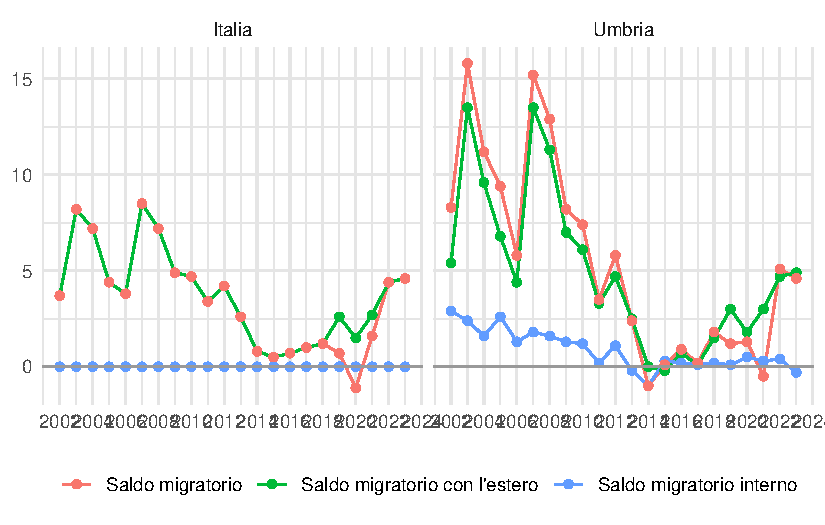
\includegraphics[keepaspectratio]{Mattioli_tesina_files/figure-pdf/Migrazione - serie storica-1.pdf}}

\subsection{Fecondità}\label{fecondituxe0}

\begin{Shaded}
\begin{Highlighting}[]
\NormalTok{fecdf }\SpecialCharTok{|\textgreater{}} 
  \FunctionTok{filter}\NormalTok{(var }\SpecialCharTok{==} \StringTok{\textquotesingle{}Tasso di fecondità totale, madri italiane\textquotesingle{}}
         \SpecialCharTok{|}\NormalTok{ var }\SpecialCharTok{==} \StringTok{\textquotesingle{}Tasso di fecondità totale, madri straniere\textquotesingle{}}
         \SpecialCharTok{|}\NormalTok{ var }\SpecialCharTok{==} \StringTok{\textquotesingle{}Tasso di fecondità totale, tutte le madri\textquotesingle{}}\NormalTok{) }\SpecialCharTok{|\textgreater{}} 
  \FunctionTok{mutate}\NormalTok{(}\AttributeTok{var =} \FunctionTok{gsub}\NormalTok{(}\StringTok{\textquotesingle{}Tasso di fecondità totale, \textquotesingle{}}\NormalTok{, }\StringTok{\textquotesingle{}\textquotesingle{}}\NormalTok{, var, }\AttributeTok{fixed =}\NormalTok{ T)) }\SpecialCharTok{|\textgreater{}} 
  \FunctionTok{ggplot}\NormalTok{(}\FunctionTok{aes}\NormalTok{(}\AttributeTok{x =}\NormalTok{ anno, }\AttributeTok{y =}\NormalTok{ value, }\AttributeTok{col =}\NormalTok{ var)) }\SpecialCharTok{+}
  \FunctionTok{geom\_line}\NormalTok{() }\SpecialCharTok{+}
  \FunctionTok{geom\_point}\NormalTok{() }\SpecialCharTok{+}
  \FunctionTok{labs}\NormalTok{(}\AttributeTok{title =} \StringTok{\textquotesingle{}Tasso di fecondità totale\textquotesingle{}}\NormalTok{) }\SpecialCharTok{+}
  \FunctionTok{scale\_x\_continuous}\NormalTok{(}\AttributeTok{breaks =} \FunctionTok{c}\NormalTok{(}\DecValTok{2002}\NormalTok{, }\DecValTok{2004}\NormalTok{, }\DecValTok{2006}\NormalTok{, }\DecValTok{2008}\NormalTok{, }\DecValTok{2010}\NormalTok{, }\DecValTok{2012}\NormalTok{, }\DecValTok{2014}\NormalTok{, }\DecValTok{2016}\NormalTok{, }\DecValTok{2018}\NormalTok{, }\DecValTok{2020}\NormalTok{, }\DecValTok{2022}\NormalTok{, }\DecValTok{2024}\NormalTok{)) }\SpecialCharTok{+}
  \FunctionTok{facet\_wrap}\NormalTok{(}\SpecialCharTok{\textasciitilde{}}\NormalTok{Territorio) }\SpecialCharTok{+}
  \FunctionTok{theme}\NormalTok{(}\AttributeTok{legend.position =} \StringTok{\textquotesingle{}bottom\textquotesingle{}}\NormalTok{,}
        \AttributeTok{panel.background =} \FunctionTok{element\_blank}\NormalTok{(),}
        \AttributeTok{panel.grid =} \FunctionTok{element\_line}\NormalTok{(}\AttributeTok{colour =} \StringTok{\textquotesingle{}gray90\textquotesingle{}}\NormalTok{),}
        \AttributeTok{legend.title =} \FunctionTok{element\_blank}\NormalTok{(),}
        \AttributeTok{strip.background =} \FunctionTok{element\_blank}\NormalTok{(),}
        \AttributeTok{axis.ticks =} \FunctionTok{element\_blank}\NormalTok{(),}
        \AttributeTok{axis.title =} \FunctionTok{element\_blank}\NormalTok{())}
\end{Highlighting}
\end{Shaded}

\pandocbounded{\includegraphics[keepaspectratio]{Mattioli_tesina_files/figure-pdf/Tasso di fecondità totale-1.pdf}}

\begin{Shaded}
\begin{Highlighting}[]
\NormalTok{fecdf }\SpecialCharTok{|\textgreater{}} 
  \FunctionTok{filter}\NormalTok{(var }\SpecialCharTok{==} \StringTok{\textquotesingle{}Età media al parto, madri italiane\textquotesingle{}}
         \SpecialCharTok{|}\NormalTok{ var }\SpecialCharTok{==} \StringTok{\textquotesingle{}Età media al parto, madri straniere\textquotesingle{}}
         \SpecialCharTok{|}\NormalTok{ var }\SpecialCharTok{==} \StringTok{\textquotesingle{}Età media al parto, tutte le madri\textquotesingle{}}\NormalTok{) }\SpecialCharTok{|\textgreater{}} 
  \FunctionTok{mutate}\NormalTok{(}\AttributeTok{var =} \FunctionTok{gsub}\NormalTok{(}\StringTok{\textquotesingle{}Età media al parto, \textquotesingle{}}\NormalTok{, }\StringTok{\textquotesingle{}\textquotesingle{}}\NormalTok{, var, }\AttributeTok{fixed =}\NormalTok{ T)) }\SpecialCharTok{|\textgreater{}} 
  \FunctionTok{ggplot}\NormalTok{(}\FunctionTok{aes}\NormalTok{(}\AttributeTok{x =}\NormalTok{ anno, }\AttributeTok{y =}\NormalTok{ value, }\AttributeTok{col =}\NormalTok{ var)) }\SpecialCharTok{+}
  \FunctionTok{geom\_line}\NormalTok{() }\SpecialCharTok{+}
  \FunctionTok{geom\_point}\NormalTok{() }\SpecialCharTok{+}
  \FunctionTok{labs}\NormalTok{(}\AttributeTok{title =} \StringTok{\textquotesingle{}Età media al parto\textquotesingle{}}\NormalTok{) }\SpecialCharTok{+}
  \FunctionTok{scale\_x\_continuous}\NormalTok{(}\AttributeTok{breaks =} \FunctionTok{c}\NormalTok{(}\DecValTok{2002}\NormalTok{, }\DecValTok{2004}\NormalTok{, }\DecValTok{2006}\NormalTok{, }\DecValTok{2008}\NormalTok{, }\DecValTok{2010}\NormalTok{, }\DecValTok{2012}\NormalTok{, }\DecValTok{2014}\NormalTok{, }\DecValTok{2016}\NormalTok{, }\DecValTok{2018}\NormalTok{, }\DecValTok{2020}\NormalTok{, }\DecValTok{2022}\NormalTok{, }\DecValTok{2024}\NormalTok{)) }\SpecialCharTok{+}
  \FunctionTok{facet\_wrap}\NormalTok{(}\SpecialCharTok{\textasciitilde{}}\NormalTok{Territorio) }\SpecialCharTok{+}
  \FunctionTok{theme}\NormalTok{(}\AttributeTok{legend.position =} \StringTok{\textquotesingle{}bottom\textquotesingle{}}\NormalTok{,}
        \AttributeTok{panel.background =} \FunctionTok{element\_blank}\NormalTok{(),}
        \AttributeTok{panel.grid =} \FunctionTok{element\_line}\NormalTok{(}\AttributeTok{colour =} \StringTok{\textquotesingle{}gray90\textquotesingle{}}\NormalTok{),}
        \AttributeTok{legend.title =} \FunctionTok{element\_blank}\NormalTok{(),}
        \AttributeTok{strip.background =} \FunctionTok{element\_blank}\NormalTok{(),}
        \AttributeTok{axis.ticks =} \FunctionTok{element\_blank}\NormalTok{(),}
        \AttributeTok{axis.title =} \FunctionTok{element\_blank}\NormalTok{())}
\end{Highlighting}
\end{Shaded}

\pandocbounded{\includegraphics[keepaspectratio]{Mattioli_tesina_files/figure-pdf/Età media al parto-1.pdf}}

\subsection{Mortalità}\label{mortalituxe0}

\begin{Shaded}
\begin{Highlighting}[]
\DocumentationTok{\#\# Speranza di vita alla nascita per sesso}
\NormalTok{umbe0 }\OtherTok{\textless{}{-}}\NormalTok{ umbMort }\SpecialCharTok{|\textgreater{}} 
  \FunctionTok{filter}\NormalTok{(Sesso }\SpecialCharTok{==} \StringTok{\textquotesingle{}Maschi\textquotesingle{}} \SpecialCharTok{\&}\NormalTok{ Età }\SpecialCharTok{==} \DecValTok{0} \SpecialCharTok{|}\NormalTok{ Sesso }\SpecialCharTok{==} \StringTok{\textquotesingle{}Femmine\textquotesingle{}} \SpecialCharTok{\&}\NormalTok{ Età }\SpecialCharTok{==} \DecValTok{0}\NormalTok{) }\SpecialCharTok{|\textgreater{}} 
  \FunctionTok{ggplot}\NormalTok{(}\FunctionTok{aes}\NormalTok{(}\AttributeTok{x =}\NormalTok{ anno, }\AttributeTok{y =} \StringTok{\textasciigrave{}}\AttributeTok{Speranza di vita}\StringTok{\textasciigrave{}}\NormalTok{, }\AttributeTok{col =}\NormalTok{ Sesso,}
             \AttributeTok{dataid =}\NormalTok{ anno, }\AttributeTok{tooltip =} \StringTok{\textasciigrave{}}\AttributeTok{Speranza di vita}\StringTok{\textasciigrave{}}\NormalTok{)) }\SpecialCharTok{+}
  \FunctionTok{geom\_point\_interactive}\NormalTok{() }\SpecialCharTok{+}
  \FunctionTok{geom\_path}\NormalTok{(}\FunctionTok{aes}\NormalTok{(}\AttributeTok{group =}\NormalTok{ Sesso)) }\SpecialCharTok{+}
  \FunctionTok{labs}\NormalTok{(}\AttributeTok{title =} \StringTok{\textquotesingle{}Speranza di vita alla nascita\textquotesingle{}}\NormalTok{,}
       \AttributeTok{subtitle =} \StringTok{\textquotesingle{}Regione Umbria\textquotesingle{}}\NormalTok{) }\SpecialCharTok{+}
  \FunctionTok{theme}\NormalTok{(}\AttributeTok{legend.position =} \StringTok{\textquotesingle{}bottom\textquotesingle{}}\NormalTok{,}
        \AttributeTok{panel.background =} \FunctionTok{element\_blank}\NormalTok{(),}
        \AttributeTok{panel.grid =} \FunctionTok{element\_line}\NormalTok{(}\AttributeTok{colour =} \StringTok{\textquotesingle{}gray90\textquotesingle{}}\NormalTok{),}
        \AttributeTok{legend.title =} \FunctionTok{element\_blank}\NormalTok{(),}
        \AttributeTok{axis.ticks =} \FunctionTok{element\_blank}\NormalTok{(),}
        \AttributeTok{axis.title =} \FunctionTok{element\_blank}\NormalTok{())}

\DocumentationTok{\#\# Speranza di vita a 65 anni per sesso}
\NormalTok{umbe65 }\OtherTok{\textless{}{-}}\NormalTok{ umbMort }\SpecialCharTok{|\textgreater{}} 
  \FunctionTok{filter}\NormalTok{(Sesso }\SpecialCharTok{==} \StringTok{\textquotesingle{}Maschi\textquotesingle{}} \SpecialCharTok{\&}\NormalTok{ Età }\SpecialCharTok{==} \DecValTok{65} \SpecialCharTok{|}\NormalTok{ Sesso }\SpecialCharTok{==} \StringTok{\textquotesingle{}Femmine\textquotesingle{}} \SpecialCharTok{\&}\NormalTok{ Età }\SpecialCharTok{==} \DecValTok{65}\NormalTok{) }\SpecialCharTok{|\textgreater{}} 
  \FunctionTok{ggplot}\NormalTok{(}\FunctionTok{aes}\NormalTok{(}\AttributeTok{x =}\NormalTok{ anno, }\AttributeTok{y =} \StringTok{\textasciigrave{}}\AttributeTok{Speranza di vita}\StringTok{\textasciigrave{}}\NormalTok{, }\AttributeTok{col =}\NormalTok{ Sesso,}
             \AttributeTok{dataid =}\NormalTok{ anno, }\AttributeTok{tooltip =} \StringTok{\textasciigrave{}}\AttributeTok{Speranza di vita}\StringTok{\textasciigrave{}}\NormalTok{)) }\SpecialCharTok{+}
  \FunctionTok{geom\_point\_interactive}\NormalTok{() }\SpecialCharTok{+}
  \FunctionTok{geom\_path}\NormalTok{(}\FunctionTok{aes}\NormalTok{(}\AttributeTok{group =}\NormalTok{ Sesso)) }\SpecialCharTok{+}
  \FunctionTok{labs}\NormalTok{(}\AttributeTok{title =} \StringTok{\textquotesingle{}Speranza di vita a 65 anni\textquotesingle{}}\NormalTok{,}
       \AttributeTok{subtitle =} \StringTok{\textquotesingle{}Regione Umbria\textquotesingle{}}\NormalTok{) }\SpecialCharTok{+}
  \FunctionTok{theme}\NormalTok{(}\AttributeTok{legend.position =} \StringTok{\textquotesingle{}bottom\textquotesingle{}}\NormalTok{,}
        \AttributeTok{panel.background =} \FunctionTok{element\_blank}\NormalTok{(),}
        \AttributeTok{panel.grid =} \FunctionTok{element\_line}\NormalTok{(}\AttributeTok{colour =} \StringTok{\textquotesingle{}gray90\textquotesingle{}}\NormalTok{),}
        \AttributeTok{legend.title =} \FunctionTok{element\_blank}\NormalTok{(),}
        \AttributeTok{axis.ticks =} \FunctionTok{element\_blank}\NormalTok{(),}
        \AttributeTok{axis.title =} \FunctionTok{element\_blank}\NormalTok{())}

\DocumentationTok{\#\# Probabilità di morte alla nascita per sesso}
\NormalTok{umbq0 }\OtherTok{\textless{}{-}}\NormalTok{ umbMort }\SpecialCharTok{|\textgreater{}} 
  \FunctionTok{filter}\NormalTok{(Sesso }\SpecialCharTok{==} \StringTok{\textquotesingle{}Maschi\textquotesingle{}} \SpecialCharTok{\&}\NormalTok{ Età }\SpecialCharTok{==} \DecValTok{0} \SpecialCharTok{|}\NormalTok{ Sesso }\SpecialCharTok{==} \StringTok{\textquotesingle{}Femmine\textquotesingle{}} \SpecialCharTok{\&}\NormalTok{ Età }\SpecialCharTok{==} \DecValTok{0}\NormalTok{) }\SpecialCharTok{|\textgreater{}} 
  \FunctionTok{ggplot}\NormalTok{(}\FunctionTok{aes}\NormalTok{(}\AttributeTok{x =}\NormalTok{ anno, }\AttributeTok{y =} \StringTok{\textasciigrave{}}\AttributeTok{Probabilità di morte (per mille)}\StringTok{\textasciigrave{}}\NormalTok{,}
             \AttributeTok{col =}\NormalTok{ Sesso, }\AttributeTok{dataid =}\NormalTok{ anno, }\AttributeTok{tooltip =} \StringTok{\textasciigrave{}}\AttributeTok{Probabilità di morte (per mille)}\StringTok{\textasciigrave{}}\NormalTok{)) }\SpecialCharTok{+}
  \FunctionTok{geom\_point\_interactive}\NormalTok{() }\SpecialCharTok{+}
  \FunctionTok{geom\_path}\NormalTok{(}\FunctionTok{aes}\NormalTok{(}\AttributeTok{group =}\NormalTok{ Sesso)) }\SpecialCharTok{+}
  \FunctionTok{labs}\NormalTok{(}\AttributeTok{title =} \StringTok{\textquotesingle{}Probabilità di morte alla nascita\textquotesingle{}}\NormalTok{,}
       \AttributeTok{subtitle =} \StringTok{\textquotesingle{}Regione Umbria\textquotesingle{}}\NormalTok{) }\SpecialCharTok{+}
  \FunctionTok{theme}\NormalTok{(}\AttributeTok{legend.position =} \StringTok{\textquotesingle{}bottom\textquotesingle{}}\NormalTok{,}
        \AttributeTok{panel.background =} \FunctionTok{element\_blank}\NormalTok{(),}
        \AttributeTok{panel.grid =} \FunctionTok{element\_line}\NormalTok{(}\AttributeTok{colour =} \StringTok{\textquotesingle{}gray90\textquotesingle{}}\NormalTok{),}
        \AttributeTok{legend.title =} \FunctionTok{element\_blank}\NormalTok{(),}
        \AttributeTok{axis.ticks =} \FunctionTok{element\_blank}\NormalTok{(),}
        \AttributeTok{axis.title =} \FunctionTok{element\_blank}\NormalTok{())}

\DocumentationTok{\#\# Patchwork}
\DocumentationTok{\#\#\# Umbria}
\NormalTok{umbe0 }\SpecialCharTok{+}\NormalTok{ umbe65 }\SpecialCharTok{+}\NormalTok{ umbq0}
\end{Highlighting}
\end{Shaded}

\pandocbounded{\includegraphics[keepaspectratio]{Mattioli_tesina_files/figure-pdf/Mortalità-1.pdf}}




\end{document}
